\chapter{Thread Creation}

This chapter describes the process and hardware involved with creating threads in the form of families of threads. The thread creation process starts when the software decides, at some point, to create a family of threads. The steps to create a family of threads are:
\begin{enumerate}
\item Obtain a place identifier to identify the place where the family should be created.
\item Allocate a context on the cores on the place.
\item Set up the allocated contexts with the index sequence and program counter.
\item ``Create'' the family; the threads in family can now be created.
\end{enumerate}

The sections below describe these actions in detail.

\section{\label{sec:place-identifier}Place identifier}
\subsection{Overview}
First, the program must decide \emph{where} to create the family. A microgrid consists of many cores, each of which can be the target of a create. The program constructs a place identifier, which is the address of the core to create to, and the number of cores to create the family on. This place identifier is obtained through an unspecified means (e.g., a software library responsible for allocating cores to applications). Figure~\ref{fig:place-contents} shows the contents of the place identifier. The place identifier is meant to fit in a single register. Its contents are:
\begin{itemize}
\item {\bf PID/Size}. These bits identify both the address and size of the place to create at. The addressing scheme is implementation-dependent but should model a linear chain of consecutive cores.
\item {\bf Capability}. These bits, the number of which depends on the implementation, make up a value which must be matched with the destination core's configured security value. This value is used to ensure that only an authorized application can perform delegated creates to certain cores.
\end{itemize}

A special place identifier value, of all 0s, is used to signal a ``default'' place. The default place is the same place as the thread that issues the allocate. I.e., when the place identifier is 0, the place identifier of the thread is used.

\begin{figure}
 \begin{center}
  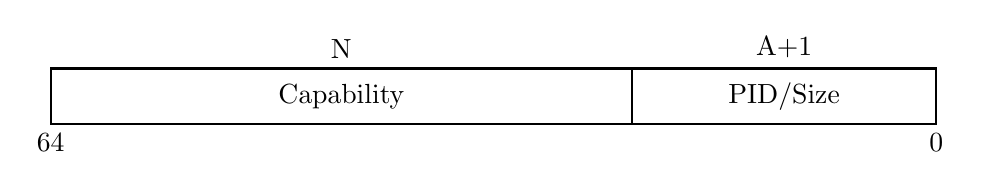
\begin{tikzpicture}[auto,thick,text badly centered]

	\begin{scope}[every node/.style={draw,rectangle,outer sep=0cm,minimum height=2em}]
		\node[minimum width=21.0em] (capability) {Capability};
		\node[minimum width=11.0em] (pidsize) at (capability.east) [right] {PID/Size};
	\end{scope}
	
	\node at (capability.north) [above] {N};
	\node at (pidsize.north) [above] {A+1};
	
	\node at (pidsize.south east) [below] {0};
	\node at (capability.south west) [below] {64};
	
\end{tikzpicture}
  \caption{Contents of a place identifier. From left-to-right: capability, exact, place address and size.}
  \label{fig:place-contents}
 \end{center}
\end{figure}

\subsection{\label{sec:pid-size}PID/Size}
The address and size of a place on a grid of $2^A$ cores are encoded in $A+1$ bits in the place identifier. Specifically, the encoding is defined as follows:
\begin{verbatim}
Encode(PID,Size) = PID * 2 + Size
\end{verbatim}
This encoding requires that {\tt Size} is a power of two and that {\tt PID} is a multiple of {\tt Size}. The former requirement ensures that the hardware can calculate thread distributions with simple shifts instead of complex divisions. The latter requirement enables this encoding, which allows for efficient distribution of families of threads over a place by software without implementation-dependent knowledge or library calls.

The PID/Size field is decoded as follows: the index (starting from the least significant bit) of the first '1' bit indicates the ($\log_2$ of the) size of the place. This bit is then cleared and the PID/Size field shifted right by 1 to obtain the place address.

Listed below are some simple operations to create a sub-place identifier from an existing place identifier ({\tt PID}). The ($\log_2$ of the) size of the input place ({\tt Size}) can be found with a single bit scan instruction.
\begin{itemize}
\item Lower half of the place: {\tt PID - Size/2}
\item Upper half of the place: {\tt PID + Size/2}
\end{itemize}

Note that none of these operations require knowledge of $A$, the number of bits that the {\tt PID/Size} is encoded in.

\section{\label{sec:family-allocation}Family allocation}

\begin{figure}
 \begin{center}
  \begin{tikzpicture}[auto,>=stealth,thick,text badly centered,component/.style={draw,rectangle,minimum height=2ex}]

	\node[component] (network) {Network};
	
	\node[draw,rectangle,minimum width=0.4cm,minimum height=1cm] (faqs) at (network) [above=1.2cm] {};
	\draw ($0.25*(faqs.south west) + 0.75*(faqs.north west)$) -- +(0.4,0);
	\draw ($0.50*(faqs.south west) + 0.50*(faqs.north west)$) -- +(0.4,0);
	\draw ($0.75*(faqs.south west) + 0.25*(faqs.north west)$) -- +(0.4,0);
	
	\node[draw,rectangle,minimum width=0.4cm,minimum height=1cm] (faqns) at (faqs.east) [right=0.1cm] {};
	\draw ($0.25*(faqns.south west) + 0.75*(faqns.north west)$) -- +(0.4,0);
	\draw ($0.50*(faqns.south west) + 0.50*(faqns.north west)$) -- +(0.4,0);
	\draw ($0.75*(faqns.south west) + 0.25*(faqns.north west)$) -- +(0.4,0);

	\node[draw,rectangle,minimum width=0.4cm,minimum height=1cm] (faqex) at (faqs.west) [left=0.1cm] {};
	\draw ($0.25*(faqex.south west) + 0.75*(faqex.north west)$) -- +(0.4,0);
	\draw ($0.50*(faqex.south west) + 0.50*(faqex.north west)$) -- +(0.4,0);
	\draw ($0.75*(faqex.south west) + 0.25*(faqex.north west)$) -- +(0.4,0);
	
	\node at (faqns.east) [right] {allocation queues};
	
	\coordinate (faqsplit) at ($(faqs.south) + (0,-0.5)$);
		
	\draw (network.north) -- (faqsplit);
	\draw[->] (faqsplit) -- (faqs.south);
	\draw[->] (faqsplit) -| node[right] {allocation requests} (faqns.south);
	\draw[->] (faqsplit) -| (faqex.south);
	
	\coordinate (faqmerge) at ($(faqs.north) + (0,0.4)$);
	\draw (faqs.north) |- (faqmerge);
	\draw (faqns.north) |- (faqmerge);
	\draw (faqex.north) |- (faqmerge);

	\node [draw, circle] (p_allocate) at (faqmerge) [above=0.4cm] {};
	\draw[->] (faqmerge) -- (p_allocate);

	\node[component] (ft) at (p_allocate) [right=1cm] {Family Table};
	\node[component] (contexts) at (p_allocate) [above=0.75cm] {Context Mgr.};
	
	\draw[<->] (p_allocate) -- (ft);
	\draw[<->] (p_allocate) -- (contexts);

	\draw[->] (p_allocate) -- +(-1.5,0) |- node[above left] {allocation responses} (network);

\end{tikzpicture}
  \caption{Overview of the components involved with the family allocation process.}
  \label{fig:family-allocation}
 \end{center}
\end{figure}

\begin{figure}
 \begin{center}
  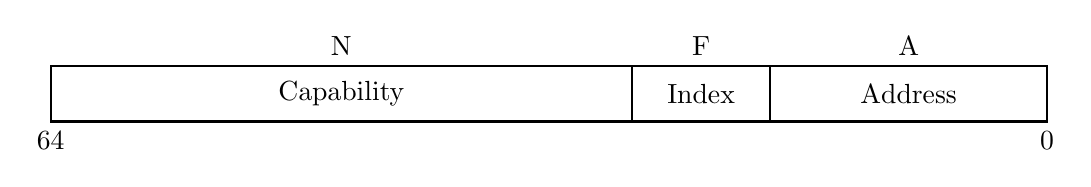
\begin{tikzpicture}[auto,thick,text badly centered]

	\begin{scope}[every node/.style={draw,rectangle,outer sep=0cm,minimum height=2em}]
		\node[minimum width=21.0em] (capability) {Capability};
		\node[minimum width=5.0em] (idx) at (capability.east) [right] {Index};
		\node[minimum width=10.0em] (pid) at (idx.east) [right] {Address};
	\end{scope}
	
	\node at (capability.north) [above] {N};
	\node at (idx.north) [above] {F};
	\node at (pid.north) [above] {A};
	
	\node at (pid.south east) [below] {0};
	\node at (capability.south west) [below] {64};
	
\end{tikzpicture}
  \caption{Contents of a family identifier. From left-to-right: capability, family index, core address.}
  \label{fig:fid-contents}
 \end{center}
\end{figure}

After a program has composed a place identifier, this is given to the {\tt Allocate} instruction. This instruction decodes the place identifier and sends an allocation request to the target core, which might be the same as the core the instruction is executed on. Eventually, the network controller on the target core handles the allocation request. The result of an allocation request is an allocation response, which writes a \emph{family ID} into the register specified by the {\tt Allocate} instruction. A family ID, as illustrated in figure~\ref{fig:fid-contents}, consists of the allocated family's index in the family table, the family's capability and the core address. Thus, the family ID provides global access to the allocated family. The capability exists to only allow access to the family entry to whoever holds the correct family ID.

Note that the number of bits for the family index and capability may depend on the core address. This allows for a heterogeneous system where certain cores have differently sized family tables. As a result, assuming that not every core knows about the architectural properties of other cores on the system, the FID should only be decoded on the core indicated by the core address. Other cores should only look at the core address part of the FID to determine whether to unpack the FID and act on it locally or send a message with the FID \emph{as-is} to the specified core.

Figure~\ref{fig:family-allocation} shows an overview of the components on a core involved with family allocation.

\subsection{Allocation queue}
\begin{figure}
 \begin{center}
  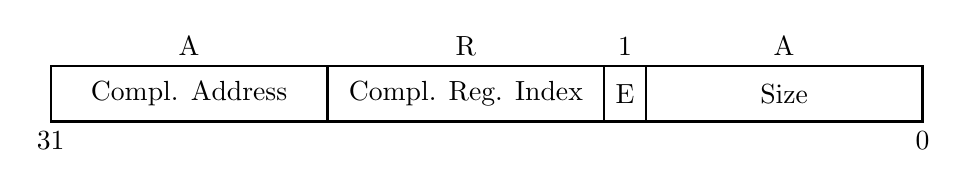
\begin{tikzpicture}[auto,thick,text badly centered]

	\begin{scope}[every node/.style={draw,rectangle,outer sep=0cm,minimum height=2em}]
		\node[minimum width=10.0em] (compl_a) {Compl. Address};
		\node[minimum width=10.0em] (compl_r) at (compl_a.east) [right] {Compl. Reg. Index};
		\node[minimum width=1.5em]  (exact) at (compl_r.east) [right] {E};
		\node[minimum width=10.0em] (size) at (exact.east) [right] {Size};
	\end{scope}
	
	\node at (compl_a.north) [above] {A};
	\node at (compl_r.north) [above] {R};
	\node at (exact.north) [above] {1};
	\node at (size.north) [above] {A};
	
	\node at (size.south east) [below] {0};
	\node at (compl_a.south west) [below] {31};
	
\end{tikzpicture}
  \caption{Contents of an entry in the allocation queue. From left-to-right: completion core address, completion register index, exact and place size.}
  \label{fig:alloc-queue-contents}
 \end{center}
\end{figure}

Once an allocation request arrives on a target core, it is simply placed in one of three queues. The three queues represent different kinds of allocation requests (implemented with three different instructions, or instruction modifiers, see chapter~\ref{chapter:isa}), neither of which should stall the other kinds. The three kinds are:
\begin{itemize}
\item {\bf Suspend}. If no context can be allocated, wait until a context is available.
\item {\bf Non-Suspend}. If no context can be allocated, return a failure code.
\item {\bf Exclusive}. Allocate the exclusive context or wait until it is available.
\end{itemize}

In case of the Non-Suspend queue, if the context manager indicates that not enough resources are available for a single context, the allocation request cannot continue. In this case, an allocation response with a failure code (a family ID of all 0s) is returned. Thus, if the program issued an Non-Suspend {\tt Allocate} instruction, it should always test the returned family ID from the instruction. 

Figure~\ref{fig:alloc-queue-contents} shows what information is stored on the allocation queue for a single allocation. The {\tt Size} and {\tt Exact} fields are taken from the place identifier and describe how many cores should be allocated for this family. The two completion fields make up a globally unique register identifier to identify where the family ID should be written to when the allocation succeeds (or fails, for Non-Suspend allocates).

A hardware process is responsible for handling the suspended allocation requests on these queues. It does this by checking the context manager if there is a free context, and allocating it if there is. If no context is available, an entry is removed from the Non-Suspend queue and {\tt failure} written back to its completion register. 

\subsection{Place allocation}

\begin{figure}
 \begin{center}
  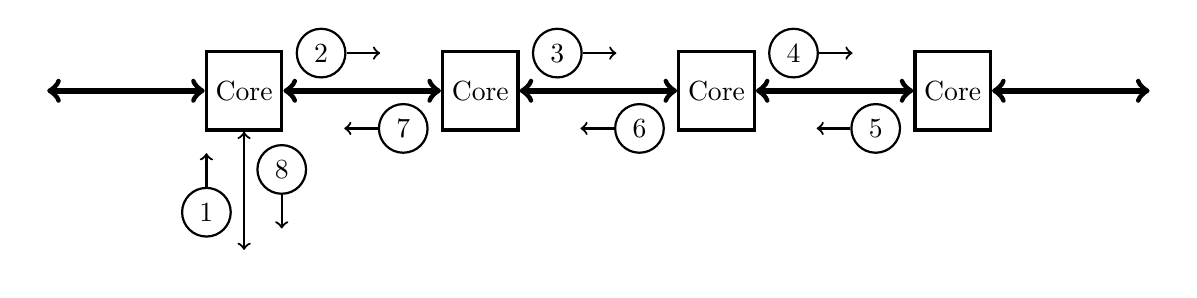
\begin{tikzpicture}[auto,thick,text badly centered]

	\node (pl) {};
	\begin{scope}[every node/.style={draw,rectangle,minimum height=1cm, very thick}]
		\node (p0) at (pl.east) [right=2cm] {Core};
		\node (p1) at (p0.east) [right=2cm] {Core};
		\node (p2) at (p1.east) [right=2cm] {Core};
		\node (p3) at (p2.east) [right=2cm] {Core};
	\end{scope}
	\node (pr) at (p3.east) [right=2cm] {};
	\node (sender) at (p0.south) [below=1.5cm] {};
	
	\begin{scope}[every node/.style={draw,circle}]
		\draw[<->] (sender) -- (p0);
		\begin{scope}[line width=2pt]
			\draw[<->] (pl) -- (p0);
			\draw[<->] (p0) -- (p1);
			\draw[<->] (p1) -- (p2);
			\draw[<->] (p2) -- (p3);
			\draw[<->] (p3) -- (pr);
		\end{scope}

		\node (s1) at (sender.north) [above left=0.25cm] {1};
		\node (s2) at (p0.east) [above right=0.25cm] {2};
		\node (s3) at (p1.east) [above right=0.25cm] {3};
		\node (s4) at (p2.east) [above right=0.25cm] {4};
		\node (s5) at (p3.west) [below left=0.25cm] {5};
		\node (s6) at (p2.west) [below left=0.25cm] {6};
		\node (s7) at (p1.west) [below left=0.25cm] {7};
		\node (s8) at (p0.south) [below right=0.25cm] {8};
		
		\draw[->] (s1) -- +(0,0.75);
		\draw[->] (s2) -- +(0.75,0);
		\draw[->] (s3) -- +(0.75,0);
		\draw[->] (s4) -- +(0.75,0);
		\draw[->] (s5) -- +(-0.75,0);
		\draw[->] (s6) -- +(-0.75,0);
		\draw[->] (s7) -- +(-0.75,0);
		\draw[->] (s8) -- +(0,-0.75);
	\end{scope}
	
\end{tikzpicture}
  \caption{Place allocation process.}
  \label{fig:place-allocation}
 \end{center}
\end{figure}

The next step, after allocating a free context depends on the place size as indicated in the place identifier. If only a single core was to be allocated, the allocation process constructs the family ID for the allocation family entry and sends a network message to write this family ID to the completion register.

However, if the place spans multiple (consecutive) cores, a message is sent to the next core (over the link network for performance, see section~\ref{sec:}) with the allocation details. Once received at the next core, the request is queued in the suspend or non-suspend allocation queue as well and handled by the allocation process.

As long as a context can be allocated, this process continues until a context has been allocated on the last core in the place. At this point, a {\tt Commit} message is sent back (over the link network) which sets up the {\tt link} field in each core's family entry to point to the corresponding family entry on the next core. Once this message returns to the beginning of the place, a network message is sent to write the family ID back to the completion register.

If, however, at some point, a context could not be allocated, and the exact flag is not set, an {\tt Unwind} message is sent backwards, freeing up allocated contexts. When enough contexts have been freed to make the number of remaining allocated contexts a power of two, the unwind message continues as a commit message. This protocol effectively allocates a smaller place than requested (if the {\tt Exact} flag is not set).

This process is illustrated in figure~\ref{fig:place-allocation}. Message 1 indicates the first allocation request coming in from the network. Messages 2--4 are allocation requests sent across the place over the link network. After the last core has allocated an entry in response to message 4, it returns a commit message which moves back over the link (messages 5--7). Once it has arrived back at the first core, an allocation response is sent back over the network.

\subsection{Context management}
The context manager maintains a count of free resources on the core, consisting of register blocks, thread entries and family entries. A context consists of one of each, and is sufficient to execute a family, one thread at a time.
There are three kinds of contexts:
\begin{itemize}
\item {\bf Free}. These contexts can be allocated or reserved for non-exclusive allocates.
\item {\bf Reserved}. A conceptual group whose contexts have been reserved for later use. Family entries never exist in this group, as they are either allocated or not. However, once a family entry is allocated, a thread entry and register block are moved to the reserved group. Note that it is strictly speaking not necessary to maintain an actual count of these contexts, assuming the allocation protocol works correctly.
\item {\bf Exclusive}. This is a single context that exists to guarantee that a core will always have a single context available for executing exclusive families. Non-exclusive allocates cannot use this context.
\end{itemize}

Only when all three counters of the desired context kind are non-zero can the allocation succeed. When this is the case, all counters are decremented by one, in essence allocating enough resources for the new family to be able to run at least one thread at a time. A family entry is allocated as well, and initialized with a (pseudo-)random security value (``capability'').

\section{\label{sec:family-setup}Family setup}
After the application has obtained a valid family ID from the allocation process, it can optionally override the index sequence and block size, whose values default values (after the family has been allocated) are set to create a family of one thread, as follows: start = 0, limit = 1, step = 1, block = 0.

\subsection{Index sequence}
The family's index sequence, determining how many threads are created, and which index values are given to those threads, is set with the {\tt setstart}, {\tt setlimit} and {\tt setstep} instructions. These instructions take two arguments: the family ID and the new value of the specified family entry's start, limit or step field, respectively. Upon executing one of these instructions, the pipeline sends a network message to the destination core, which might be same core. On the destination core, the network logic handles the message and writes the value into the family entry.

The values of the start, limit and step fields are interpreted based on the value of the step field, as follows:

\vskip 2ex
\noindent\begin{tabular}{ll}
step $=$ 0: & (Invalid)\\
step $>$ 0: & {\tt for (int i = start; i < limit; i += step)}\\
step $<$ 0: & {\tt for (int i = start; i > limit; i += step)}\\
\end{tabular}
\vskip 2ex

That is, the family index is equivalent with the specified for loops, where one thread is created for each iteration, in sequence. Note that the fields, and their comparisons are \emph{signed} comparisons on integers with machine-word size.

\subsection{\label{sec:block-size}Block size}
The block size for the new family is set with the {\tt setblock} instruction (see section~\ref{sec:setblock}). The block size determines an upper bound on the number of thread entries allocated on a single core for the family, i.e., the size of the family's block of threads. This value may be further constrained by the hardware based on the availability of registers, as described in section~\ref{sec:registers-family-creation}. The block size exists to prevent an explosion of resource usage of the non-leaf nodes in the concurrency tree, by restricting the resources that those nodes use.

A block size of 0, which is the default when a family entry is allocated, indicates the maximum possible block size, i.e., the thread table size.

\section{\label{sec:family-creation}Family creation}

\begin{figure}
 \begin{center}
  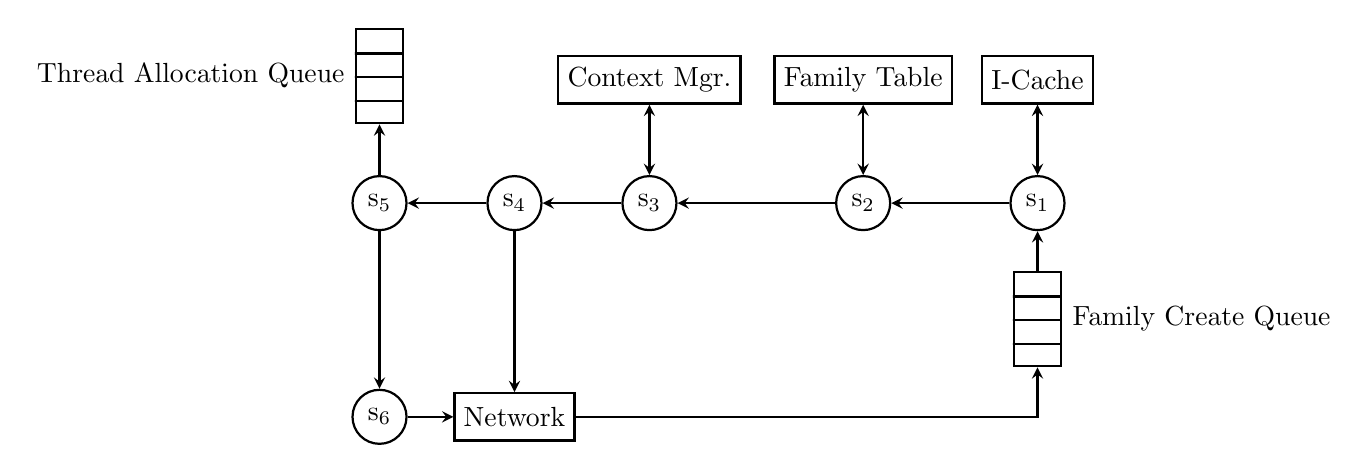
\begin{tikzpicture}[auto,>=stealth,thick,text badly centered]

  % Family allocation queue
  \node[draw,rectangle,minimum width=0.6cm,minimum height=1.2cm] (falloc) {};
  \draw (falloc.south west)+(0,0.3) rectangle +(0.6,0.3);
  \draw (falloc.south west)+(0,0.6) rectangle +(0.6,0.6);
  \draw (falloc.south west)+(0,0.9) rectangle +(0.6,0.9);
   
  \begin{scope}[every node/.style={draw,circle}]
    \node (s1) at (falloc.north) [above=0.5cm] {s$_1$};
    \node (s2) at (s1.west) [left=1.5cm] {s$_2$};
    \node (s3) at (s2.west) [left=2cm] {s$_3$};
    \node (s4) at (s3.west) [left=1cm] {s$_4$};
    \node (s5) at (s4.west) [left=1cm] {s$_5$};
    \node (s6) at (s5.south) [below=2cm] {s$_6$};
  \end{scope}
  \node at (falloc.east) [right] {Family Create Queue};
  
  \draw[->] (falloc) -- (s1);
  \draw[->] (s1) -- (s2);
  \draw[->] (s2) -- (s3);
  \draw[->] (s3) -- (s4);
  \draw[->] (s4) -- (s5);
  \draw[->] (s5) -- (s6);
  
  \begin{scope}[every node/.style={draw,rectangle,minimum height=0.6cm}]
    \node (icache)   at (s1) [above=1.25cm] {I-Cache};
    \node (ft)       at (s2) [above=1.25cm] {Family Table};
    \node (contexts) at (s3) [above=1.25cm] {Context Mgr.};
  \end{scope}
  
  % Thread allocation queue
  \node[draw,rectangle,minimum width=0.6cm,minimum height=1.2cm] (talloc) at (s5) [above=1cm] {};
  \draw (talloc.south west)+(0,0.3) rectangle +(0.6,0.3);
  \draw (talloc.south west)+(0,0.6) rectangle +(0.6,0.6);
  \draw (talloc.south west)+(0,0.9) rectangle +(0.6,0.9);
  \node at (talloc.west) [left] {Thread Allocation Queue};

  % Network
  \node[draw,rectangle,minimum height=0.6cm] (net) at (s6 -| s4) {Network};
  \draw[->] (net) -| (falloc);
  
  \begin{scope}[every node/.style={font=\footnotesize}]
    \draw[<->] (s1) -- (icache);
    \draw[<->] (s2) -- (ft);
    \draw[->]  (s4) -- (net);
    \draw[<->] (s3) -- (contexts);
    \draw[->]  (s5) -- (talloc);
    \draw[->]  (s6) -- (net);
  \end{scope}
  
\end{tikzpicture}
  \caption{Family creation process.}
  \label{fig:family-creation}
 \end{center}
\end{figure}

\begin{figure}
 \begin{center}
  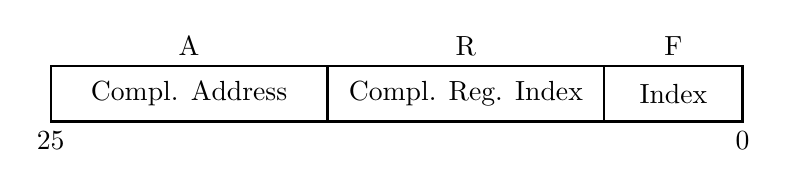
\begin{tikzpicture}[auto,thick,text badly centered]

	\begin{scope}[every node/.style={draw,rectangle,outer sep=0cm,minimum height=2em}]
		\node[minimum width=10.0em] (compl_a) {Compl. Address};
		\node[minimum width=10.0em] (compl_r) at (compl_a.east) [right] {Compl. Reg. Index};
		\node[minimum width=5.0em] (index) at (compl_r.east) [right] {Index};
	\end{scope}
	
	\node at (compl_a.north) [above] {A};
	\node at (compl_r.north) [above] {R};
	\node at (index.north) [above] {F};
	
	\node at (index.south east) [below] {0};
	\node at (compl_a.south west) [below] {25};
	
\end{tikzpicture}
  \caption{Contents of an entry in the create queue. From left-to-right: completion core address, completion register index, family index.}
  \label{fig:create-queue-contents}
 \end{center}
\end{figure}

Once a family has been allocated and initialized, the program can issue a {\tt create} instruction. This instruction takes the family ID of the setup family and a pointer into memory identifying the beginning of the family's threads' executable code.

Upon executing this instruction, the pipeline checks if there are pending writes for this thread. If so, the pipeline pretends a memory write barrier has been executed and suspends the thread on the pending writes (see section~\ref{sec:}). When the data cache acknowledges the last pending write, the thread is reschedule and the create instruction re-executed. This in effect turns family creation into an implicit write barrier, allowing earlier-made writes by the thread to be committed to memory before creating the family, which might need that data in memory.

If the create is executed and there are no pending writes, a network message with the create information is sent to the specified core. The network controller on the target core will write the code pointer and buffer the create information on that core's create queue. The buffered information is shown in figure~\ref{fig:create-queue-contents}.

The create queue is handled by a seperate process which implement a multi-stage, multi-cycle operation. This process can be implemented by a state machine or pipeline. Figure~\ref{fig:family-creation} shows this process in a pipelined form and how it interacts with the various components on the core. The stages of the process are explained next.

\subsection{Register counts}

\begin{figure}
 \begin{center}
  \begin{tikzpicture}[auto,thick,text badly centered]

	\begin{scope}[every node/.style={draw,rectangle,outer sep=0cm,minimum height=2em,font=\footnotesize}]
		\node[minimum width=1em] (dummy1) {};
		\node[minimum width=5em] (fltl) at (dummy1.east) [right] {Locals};
		\node[minimum width=5em] (flts) at (fltl.east) [right] {Shareds};
		\node[minimum width=5em] (fltg) at (flts.east) [right] {Globals};
		\node[minimum width=1em] (dummy2) at (fltg.east) [right] {};
		\node[minimum width=5em] (intl) at (dummy2.east) [right] {Locals};
		\node[minimum width=5em] (ints) at (intl.east) [right] {Shareds};
		\node[minimum width=5em] (intg) at (ints.east) [right] {Globals};
	\end{scope}
	
	\node at (fltl.north) [above] {5};
	\node at (flts.north) [above] {5};
	\node at (fltg.north) [above] {5};
	\node at (intl.north) [above] {5};
	\node at (ints.north) [above] {5};
	\node at (intg.north) [above] {5};
	
	\node at (intg.south east) [below] {0};
	\node at (fltg.south east) [below] {16};
	\node at (dummy1.south west) [below] {32};
	
	\begin{scope}[decoration=brace]
	  \draw[decorate] (intl.north west)+(0,4ex) -- node[above=1.5ex,anchor=base]{Integers} ($(intg.north east)+(0,4ex)$);
	  \draw[decorate] (fltl.north west)+(0,4ex) -- node[above=1.5ex,anchor=base]{Floats}   ($(fltg.north east)+(0,4ex)$);
	\end{scope}
	
\end{tikzpicture}
  \caption{Contents of ``register count'' word on a RISC architecture with 5-bit register specifiers and 32-bit instruction words.}
  \label{fig:reg-counts}
 \end{center}
\end{figure}

The first stage of the create process reads the entry from the front of the family allocation queue and the code pointer from the family table. It uses the code pointer to fetch the cache-line containing this code pointer through the I-Cache. This cache-line also contains the register count word for the threads of the family. The register count word is the first word before the location pointed to by the code pointer and contains the number of local, shared and global registers that should be used for each thread's virtual register context (see section~\ref{sec:registers-virtual-layout}). Figure~\ref{fig:reg-counts} shows the contents of this word. If the fetch hits the I-Cache, the family ID continues to the second stage. Otherwise, a flag is set in the I-Cache's line (see section~\ref{sec:icache-creation-flag}) which will cause the I-Cache to wake up this process and advance it to the next stage when the cache-line has been loaded.

\subsection{\label{sec:family-setup-finalization}Family setup finalization}
The next stage finalizes the family setup with the register information that was loaded in the previous stage. The shared register count is checked to determine if the family is independent (when all shared counts are 0). This information, combined with the number of cores that have been allocated to the family is used to calculate the thread distribution.

The number of threads in the family is determined from the start, limit and step fields as described earlier in this section. Based on the number of threads. The threads are evenly distributed across the allocated cores, where each core executes $\lceil \#threads / \#cores \rceil$. Should the number of threads not be an integer multiple of the number of cores, the last core executes fewer threads. Note that the number of allocated cores is always a power of two to simplify this division to a shift in hardware.

Threads of dependent families require their shareds communicated between threads. If these threads are distributed across multiple cores, the administration of keeping track of these dependencies is non-trivial. Considering, as well, that the global performance of dependent families is coupled with the size of the independent pre- of post-fix to the dependent part in the thread, the architecture does not distribute dependent families. Such families are executed on the first core, regardless of the number of cores that have been allocated. Should a dependent algorithm need to be distributed across multiple cores, a multi-family approach can be used where the top-level dependent family runs on the first core and creates a single dependent family on each of the allocated cores. The only non-local register communication is the initial and final shareds of the family.

Exclusive families, just like dependent families, execute all their threads on the first core as well.

With the number of threads and their distribution known, this stage advances the \emph{start} field in the family entry to the correct value based on the number of threads per core and the core's offset to the first core in the family. The \emph{limit} field is written with the number of threads that are left to be created on this core. Note that it thus takes on a different semantic meaning. The same field for both meanings is used to save space in the family table. This can be done because their uses are mutually exclusive.

\subsection{\label{sec:register-alloc}Register allocation}
The next step in the family create process is allocating the desired amount of registers from the register file. The context manager has an administration of available registers that is consulted to accomplish this task. Typically, the allocation granularity is not a single register, but a block of registers, at least being a single thread worth of registers. Having a larger allocation block size reduces the logic involved with allocating registers since there are fewer blocks to allocate, reduces fragmentation of the register file and makes it trivial to guarantee that a single context reservation is available as a block of consecutive registers.

The family's block size, as set by the program, is used to calculate the number of registers to allocate: {\tt \#globals + \#shareds + block\_size $\cdot$ (\#locals + \#shareds)}. This amount is rounded up to a multiple of the allocation block size and a contiguous range of registers of this size is allocated from the available registers, if possible. This is done for both the integer and floating-point registers.

If the context manager indicates that such there are not enough free registers, the block size is reduced by one, and the process is repeated. Since family allocation reserves one register context for the family, and given that {\tt \#globals + 2 $\cdot$ \#shareds + \#locals} should not be greater than a single context, this process is guaranteed to at least succeed if the block size goes down to one.

\subsection{Create distribution}
With the distribution determined and all resources allocated on this core, the next step forwards the create via the link network to the next core, if any. The message indicates the family entry index of the family on the next core (read from the family's \emph{link} field). Once received, the network controller on the next core queues the create. When it gets handled, its registers are allocated, the family pushed onto the thread allocation queue (see next section) and another create message is sent to the next core over the link network.

\subsection{Thread allocation queue}
At this point, the family is ready to start creating threads. The family index is pushed on the core's \emph{thread allocation queue}, a queue of family indices which indicate families that have been created and are ready to start executing threads. Section~\ref{sec:thread-alloc} discusses this mechanism.

\subsection{Creation notification}
To ensure that register writes from the parent and the first thread in the family do not occur when no registers have been allocated, creates are not notified until after the register have been allocated and the create has been sent to the other cores. This way, when the parent receives the create notification (i.e., the register specified at the create instruction is written), subsequent global writes sent to the first core in the family will succeed the create notification on the link network, thus ensuring that registers will always be allocated once the global write arrives.

This stage is the final stage in the family creation process.

\section{\label{sec:thread-alloc}Thread allocation}

Once a family index has been pushed onto the thread allocation queue, it means its family entry is entirely setup and enough registers have been allocated to accomodate the block size. A hardware process is responsible for allocating threads to this family.

After a family has been created on a core, its index is pushed onto the \emph{thread allocation queue}. This is a queue of families that need to have threads created for them and have fewer threads than the block size. The thread allocation hardware process continuously creates threads for the family at the head of this queue until it has reached the block size, or until the family has created all its threads.

Once a thread has terminated and its dependencies (see section~\ref{sec:thread-dependencies}) have been resolved, the thread is pushed onto the cleanup queue. Since thread cleanup results in the reuse of the thread entry, thread cleanup is essentially thread allocation. Therefore, thread cleanup is performed by the same process as thread allocation. If the core's cleanup queue is not empty, the thread allocation process pops a thread off this queue. If the thread's family does not have its thread allocated yet, the thread entry is used to allocate the next thread in the family. Otherwise, the thread entry is put on the core's empty thread list (i.e., the entry is freed).

Only if the cleanup queue is empty, does the thread allocation process look at the thread allocation queue.

After allocating (or reusing) a thread entry, it must be initialized for initial execution of the thread. This involves copying various fields from the family entry to the thread entry and updating various fields in the family table.

Note that the thread's local register offset field only has to be initialized if the thread entry is freshly allocated. Otherwise, the thread can reuse the local from the entry's previous thread.

After the thread entry is initialized, the current index of the thread (as taken from the family's \emph{start} field), is written into the first local register of the thread, if the thread has one or more local registers.

Finally, the thread is ready to be executed and its index is put on a thread ready list for the thread scheduler (see section~\ref{sec:ready-list}).